137. Нарисуйте, как из данных трёх фигурок, использовав каждую ровно один раз, сложить фигуру, имеющую ось симметрии.
\begin{center}
\begin{figure}[ht!]
\center{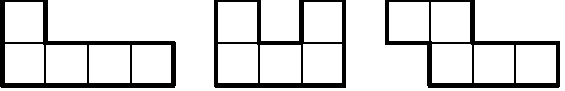
\includegraphics[scale=0.35]{34.png}}
\end{figure}
\end{center}
